 %!TEX root = ./template-skripsi.tex
%-------------------------------------------------------------------------------
%                            BAB II
%               KAJIAN TEORI
%-------------------------------------------------------------------------------

\chapter{KAJIAN PUSTAKA} 

\section{Perikanan modern}
Perikanan modern adalah pendekatan dalam industri perikanan yang melibatkan penggunaan teknologi canggih, manajemen yang efisien, dan prinsip-prinsip berkelanjutan untuk memaksimalkan produksi ikan dan produk-produk perikanan, sambil tetap menjaga keseimbangan ekosistem dan menjaga sumber daya alam \citep{kusuma2004sistem}.

Perikanan modern melibatkan penerapan teknologi seperti pemantauan satelit, sistem informasi geografis (GIS), penggunaan peralatan nirkabel, penggunaan kapal tangkap yang lebih efisien dan ramah lingkungan, pengelolaan data untuk mengoptimalkan produksi, budidaya ikan secara intensif (aquaculture), serta penerapan praktik-praktik manajemen berkelanjutan yang melibatkan perlindungan terhadap lingkungan laut, pemantauan dan pengelolaan stok ikan, serta penegakan regulasi dan kebijakan.

\section{Sistem backend yang bertanggung jawab untuk melayani transaksi query}

Sistem backend yang bertanggung jawab untuk melayani transaksi query dalam konteks pengembangan perangkat lunak sering disebut sebagai "Query Backend System" atau "Query Processing System." Ini adalah komponen yang mengelola permintaan query dari frontend (pengguna atau aplikasi) dan berinteraksi dengan basis data atau penyimpanan data untuk mengambil, memanipulasi, dan mengembalikan hasil yang relevan \citep{prayogi2021rancang}.

Fungsi utama dari Query Processing System adalah untuk menerima permintaan query (pertanyaan atau perintah) dari pengguna atau aplikasi, menganalisis query tersebut, mengeksekusi operasi yang sesuai pada basis data, dan menghasilkan hasil yang relevan. Proses ini melibatkan beberapa langkah untuk mengoptimalkan kinerja dan efisiensi eksekusi query.


\section{\emph{Scrum}}
\emph{Scrum} merupakan kerangka kerja ringan yang dapat menghasilkan solusi yang adaptif untuk masalah yang kompleks bagi orang, tim, dan organisasi. Kerangka kerja scrum dibiarkan tidak lengkap, hanya mendefinisikan bagian-bagian yang diperlukan untuk mengimplementasi teori \emph{scrum}, selebihnya kecerdasan kolektif orang-orang yang menggunakan \emph{scrum} akan membangun \emph{scrum} itu sendiri. \emph{Scrum} tidak memberikan instruksi yang terperinci kepada setiap anggota tim, melainkan memandu hubungan dan interaksi mereka.

\emph{Scrum} terus berkembang dengan adanya pengalaman dan pemikiran, lalu menghasilkan suatu keputusan berdasarkan pengamatan. Menggunakan proses iterasi dan perlahan menambahkan sesuatu, untuk mengendalikan risiko dan membuat sesuatu dapat diprediksi.

\emph{Scrum} menggunakan prinsip pendekatan \emph{Agile} untuk dapat mengatasi segala macam masalah secara kreatif dan adaptif. Berbagai proses, teknik dan metode dapat digunakan dalam kerangka kerja. 

\emph{Scrum} menggabungkan empat aktivitas formal untuk memeriksa dan mengadaptasi menjadi satu aktivitas konten, \emph{Sprint}. Kegiatan ini dapat berhasil jika menerapkan pilar empiris transparansi, inspeksi, dan adaptasi \emph{Scrum}. 

\begin{enumerate}
	\item Transparansi
	
	Proses dan pekerjaan yang muncul harus dapat dilihat oleh mereka yang melakukan pekerjaan dan mereka yang menerimanya. Untuk \emph{Scrum}, sangat penting bahwa keputusan didasarkan pada kondisi tiga komponen formal, dan komponen \emph{Scrum} dengan transparansi rendah mengurangi nilai dan meningkatkan risiko.
		
	\item Inspeksi
		
	Artefak \emph{scrum} dan kemajuan menuju tujuan yang disepakati harus dirombak secara berkala untuk mendeteksi kemungkinan perbedaan atau masalah yang tidak terduga. Untuk membantu inspeksi, \emph{Scrum} menyediakan ritme dalam bentuk lima acaranya.

	Centang untuk memungkinkan adaptasi. Inspeksi tanpa adaptasi dianggap tidak berguna. Aktivitas \emph{scrum} dirancang untuk menginspirasi perubahan.	
		
	\item Adaptasi
	
	Jika ada aspek proses yang menyimpang dari batas yang dapat diterima, atau jika produk yang dihasilkan tidak dapat diterima, proses yang diterapkan atau bahan yang dihasilkan harus disesuaikan. Penyesuaian harus dilakukan sesegera mungkin untuk meminimalkan penyimpangan lebih lanjut.

	Adaptasi menjadi lebih sulit ketika orang-orang yang terlibat tidak diberdayakan atau dikelola sendiri. Tim \emph{scrum} diharapkan untuk menyesuaikan diri saat mereka mempelajari hal-hal baru melalui inspeksi.

\end{enumerate}

	\subsection{Tim Scrum}
	
	Unit dasar \emph{Scrum} adalah tim kecil. \emph{Scrum Team} terdiri dari \emph{Scrum Master}, \emph{Product Owner}, dan \emph{Developer}. Dalam tim \emph{Scrum}, tidak ada sub-tim atau hierarki. Tim \emph{scrum} bersifat lintas fungsi, yang berarti bahwa anggota memiliki semua keterampilan yang mereka butuhkan untuk menciptakan nilai di setiap \emph{Sprint}. Tim scrum cukup kecil untuk tetap lincah dan cukup besar untuk menyelesaikan pekerjaan penting dalam sprint, biasanya 10 orang atau kurang.

	Tim \emph{Scrum} bertanggung jawab atas semua aktivitas terkait produk, termasuk kolaborasi pemangku kepentingan, validasi, pemeliharaan, operasi, eksperimen, penelitian dan pengembangan, dan aktivitas lain apa pun yang mungkin diperlukan.

	Seluruh Tim \emph{Scrum} bertanggung jawab untuk menciptakan peningkatan yang berharga dan berguna di setiap \emph{Sprint}. \emph{Scrum} mendefinisikan tiga tanggung jawab khusus dalam Tim \emph{Scrum}: Pengembang, Pemilik Produk, dan \emph{Scrum Master}.
	
	\begin{enumerate}
	
		\item Pengembang (\emph{Developers})
		
		Pengembang adalah seseorang di tim \emph{Scrum} yang bekerja untuk membuat aspek apa pun dari \emph{Increment} yang dapat digunakan oleh setiap Sprint.

		Keterampilan khusus yang dibutuhkan oleh pengembang seringkali luas dan bervariasi menurut bidang pekerjaan. Namun, pengembang selalu bertanggung jawab untuk:
		
		\begin{enumerate} [a.]
		
			\item Mengembangkan rencana untuk \emph{Sprint}, \emph{Sprint Backlog};

			\item Menanamkan kualitas dengan tetap berpegang pada definisi selesai;

			\item Menyesuaikan rencana harian mereka untuk mencapai \emph{Sprint Goals}; dan,

			\item Sebagai profesional, kami memikul tanggung jawab satu sama lain.
		
		\end{enumerate}
		
		\item Pemilik Produk (\emph{Product Owner})
		
		Pemilik Produk bertanggung jawab untuk memaksimalkan nilai produk yang dikembangkan oleh Tim \emph{Scrum}. Bagaimana hal ini dicapai akan bervariasi antara perusahaan, tim, dan individu. \emph{Product Owner} juga bertanggung jawab untuk mengelola \emph{Product Backlog} dengan baik, termasuk:
		
		\begin{enumerate} [a.]
		
			\item Mengembangkan dan mengkomunikasikan tujuan produk dengan jelas;

			\item Membuat dan mengkomunikasikan item backlog produk dengan jelas; 
			
			\item Memesan backlog produk; dan,

			\item Pastikan \emph{Product Backlog} transparan, terlihat, dan mudah dipahami.
		
		\end{enumerate}
		
		Pemilik Produk dapat melakukan pekerjaan yang dijelaskan di atas atau mendelegasikan tanggung jawab kepada orang lain. Seluruh organisasi harus menghormati keputusan mereka. Keputusan ini tercermin dalam konten dan urutan \emph{Product Backlog}, dan melalui peningkatan yang dapat diperiksa di \emph{Sprint Review}.

		Pemilik Produk adalah orang, bukan panitia. Pemilik Produk dapat mewakili kebutuhan banyak pemangku kepentingan dalam \emph{Product Backlog}. Siapapun anggota tim yang ingin mengubah \emph{Product Backlog} dapat melakukannya dengan mencoba meyakinkan Pemilik Produk.
		
		\item \emph{Scrum Master}
		
		\emph{Scrum Master} bertanggung jawab untuk membangun \emph{Scrum} sebagaimana didefinisikan dalam Panduan \emph{Scrum}. Mereka melakukan ini dengan membantu semua orang di tim dan organisasi \emph{Scrum} memahami teori dan praktik \emph{Scrum}.

		\emph{Scrum Master} bertanggung jawab atas efektivitas Tim \emph{Scrum}. Mereka melakukan ini dengan meminta tim \emph{Scrum} meningkatkan praktik mereka dalam kerangka kerja \emph{Scrum}.

		\emph{Scrum Masters} adalah pemimpin sejati yang melayani Tim \emph{Scrum} dan organisasi yang lebih besar.

		\emph{Scrum Master} melayani Tim Scrum dengan cara, seperti:
		
		\begin{enumerate}[a.]
		
			\item Melatih anggota tim dalam manajemen diri dan manajemen berbagai bidang;

			\item Bantu tim \emph{Scrum} fokus pada penciptaan peningkatan bernilai tinggi yang memenuhi definisi selesai;

			\item Buka blokir kemajuan Tim \emph{Scrum}; dan,

			\item Pastikan semua acara \emph{Scrum} terjadi, positif, produktif, dan sesuai jadwal.
		
		\end{enumerate}
		
		\emph{Scrum Master} melayani Pemilik Produk dengan cara, seperti:
		
		\begin{enumerate}[a.]
		
			\item Membantu menemukan teknik untuk definisi tujuan produk yang efektif dan manajemen simpanan produk;

			\item Membantu tim \emph{Scrum} memahami kebutuhan akan item \emph{Product Backlog} yang jelas dan ringkas;

			\item Membantu membangun program produk empiris untuk lingkungan yang kompleks; dan,

			\item Memfasilitasi kolaborasi pemangku kepentingan sesuai kebutuhan atau kebutuhan.
		
		\end{enumerate}
		
		\emph{Scrum Master} melayani organisasi dengan cara, seperti:
		
		\begin{enumerate}[a.]
		
			\item Memimpin, melatih dan melatih organisasi dalam implementasi \emph{Scrum};

			\item Merencanakan dan merekomendasikan penerapan \emph{Scrum} dalam organisasi;

			\item Membantu karyawan dan pemangku kepentingan memahami dan menerapkan metode empiris untuk pekerjaan yang kompleks; dan,

			\item Menghilangkan hambatan antara \emph{stakeholder} dan tim \emph{Scrum}.
		
		\end{enumerate}


	\end{enumerate}

	\subsection{Aktivitas-aktivitas Scrum (Scrum Events)}
	
	\emph{Sprint} adalah wadah untuk semua acara lainnya. Setiap acara di \emph{Scrum} adalah kesempatan formal untuk meninjau dan menyesuaikan artefak \emph{Scrum}. Acara-acara ini secara khusus dirancang untuk mencapai transparansi yang diperlukan. Kegagalan untuk mengoperasikan acara apapun seperti yang ditentukan menghasilkan kesempatan yang hilang untuk peninjauan dan adaptasi. Acara digunakan di \emph{Scrum} untuk menciptakan ketertiban dan meminimalkan kebutuhan akan rapat yang tidak ditentukan dalam \emph{Scrum}. Idealnya, semua acara diadakan pada waktu dan tempat yang sama untuk mengurangi kerumitan.
	
	\begin{enumerate}
	
		\item \emph{Sprint}
		
		\emph{Sprint} adalah jantung dari \emph{Scrum}, di mana ide-ide diubah menjadi nilai. Mereka adalah acara berdurasi tetap satu bulan atau kurang untuk menciptakan konsistensi. \emph{Sprint} baru dimulai segera setelah \emph{Sprint} sebelumnya berakhir.

		Semua pekerjaan yang diperlukan untuk mencapai Tujuan Produk, termasuk Perencanaan \emph{Sprint}, \emph{Scrum} Harian, Ulasan \emph{Sprint}, dan Retrospektif \emph{Sprint}, terjadi selama:
		
		\begin{enumerate}[a.]
		
			\item tidak membuat perubahan apa pun yang akan membahayakan \emph{Sprint Goal};

			\item Kualitas tidak berkurang;

			\item \emph{Product Backlog} sedetail yang dibutuhkan; dan,

			\item Semakin banyak yang dipelajari, ruang lingkup dapat diklarifikasi dan dinegosiasikan ulang dengan Pemilik Produk.
		
		\end{enumerate}
		
		\emph{Sprint} memungkinkan prediktabilitas dengan memastikan bahwa kemajuan terhadap sasaran produk diperiksa dan diakomodasi setidaknya setiap bulan kalender. Ketika Cakrawala Sprint terlalu panjang, Tujuan Sprint mungkin gagal, kompleksitas dapat meningkat, dan risiko dapat meningkat. \emph{Sprint} yang lebih pendek dapat digunakan untuk menghasilkan lebih banyak siklus pembelajaran dan membatasi risiko biaya dan upaya untuk kerangka waktu yang lebih pendek. Setiap \emph{Sprint} dapat dianggap sebagai proyek pendek.

	Berbagai praktik ada untuk memprediksi kemajuan, seperti kelelahan, kelelahan, atau aliran kumulatif. Meskipun terbukti bermanfaat, ini tidak menggantikan pentingnya empirisme. Dalam lingkungan yang kompleks, apa yang terjadi tidak diketahui. Hanya apa yang telah terjadi yang dapat digunakan untuk keputusan berwawasan ke depan. \emph{Sprint} dapat dibatalkan jika \emph{Sprint Goals} sudah kedaluwarsa. Hanya Pemilik Produk yang berhak membatalkan Sprint.
		
		\item Perencanaan \emph{Sprint}
		
		Perencanaan \emph{Sprint} memulai \emph{Sprint} dengan meletakkan pekerjaan yang harus dilakukan untuk \emph{Sprint}. Rencana akhir dibuat secara kolaboratif oleh seluruh tim \emph{Scrum}.

		\emph{Product Owner} memastikan bahwa peserta siap untuk mendiskusikan item \emph{Product Backlog} yang paling penting dan bagaimana mereka memetakan ke tujuan produk. Tim \emph{Scrum} juga dapat mengundang orang lain untuk berpartisipasi dalam Perencanaan \emph{Sprint} untuk memberikan saran.
		
		\item \emph{Scrum} harian (\emph{Daily Scrum})
		
		Tujuan dari \emph{Daily Scrum} adalah untuk memeriksa kemajuan terhadap \emph{Sprint Goals} dan menyesuaikan \emph{Sprint Backlog} sesuai kebutuhan untuk menyesuaikan rencana kerja di masa mendatang.

		\emph{Daily Scrum} adalah aktivitas 15 menit untuk pengembang di tim \emph{Scrum}. Untuk mengurangi kompleksitas, ini dilakukan pada waktu dan tempat yang sama setiap hari kerja \emph{Sprint}. Jika \emph{Product Owner} atau \emph{Scrum Master} aktif mengerjakan item di \emph{Sprint Backlog}, mereka berpartisipasi sebagai \emph{developer}.

		Pengembang dapat memilih struktur dan teknik apa pun yang mereka inginkan, selama \emph{Scrum} harian mereka berfokus pada kemajuan Tujuan \emph{Sprint} dan memiliki rencana yang dapat diterapkan untuk hari kerja berikutnya. Ini menciptakan fokus dan meningkatkan manajemen diri.

		\emph{Daily Scrum} dapat meningkatkan komunikasi, mengidentifikasi hambatan, dan memfasilitasi pengambilan keputusan yang cepat, menghilangkan kebutuhan untuk rapat ulang.
		
		\emph{Daily Scrum} bukan satu-satunya waktu pengembang menyesuaikan rencana mereka. Tim sering bertemu sepanjang hari untuk berdiskusi lebih rinci tentang cara menyesuaikan atau merencanakan ulang sisa \emph{print}.
		
		\item Pembahasan \emph{Sprint} (\emph{Sprint Review})
		
		Tujuan dari \emph{Sprint Review} adalah untuk memeriksa hasil \emph{Sprint} dan mengidentifikasi penyesuaian di masa depan. Tim scrum mempresentasikan hasil kerja mereka kepada pemangku kepentingan utama dan mendiskusikan kemajuan menuju tujuan produk.

		Selama acara, Tim \emph{Scrum} dan pemangku kepentingan meninjau apa yang telah dicapai dalam \emph{Sprint} dan bagaimana lingkungan mereka telah berubah. Berdasarkan informasi ini, peserta berkolaborasi tentang apa yang harus dilakukan selanjutnya. \emph{Product Backlog} juga dapat disesuaikan untuk memenuhi peluang baru. Tinjauan \emph{Sprint} adalah rapat kerja dan Tim Scrum harus menghindari membatasinya pada presentasi.

		\emph{Sprint Review} adalah kegiatan \emph{Sprint} kedua dari belakang, dan \emph{Sprint} sebulan tidak melebihi maksimal empat jam. Acara biasanya lebih pendek untuk \emph{Sprint} yang lebih pendek.
				
		\item \emph{Sprint Retrospektif}
		
		Tujuan dari \emph{Sprint Retrospective} adalah untuk merencanakan cara-cara untuk meningkatkan kualitas dan efektivitas.

		Tim \emph{Scrum} memeriksa bagaimana \emph{Sprint} terakhir berjalan sehubungan dengan individu, interaksi, proses, alat, dan Definisi Selesai. Elemen yang diperiksa seringkali berbeda dengan domain pekerjaan. Asumsi yang menyesatkan mereka diidentifikasi dan asal-usulnya dieksplorasi. Tim \emph{Scrum} mendiskusikan apa yang berjalan dengan baik selama \emph{Sprint}, masalah apa yang dihadapi, dan bagaimana masalah tersebut (atau tidak) diselesaikan.

		Tim \emph{Scrum} mengidentifikasi perubahan yang paling membantu untuk meningkatkan efektivitasnya. Perbaikan yang paling berdampak ditangani sesegera mungkin. Mereka bahkan dapat ditambahkan ke \emph{Sprint Backlog} untuk \emph{Sprint} berikutnya.

		\emph{Sprint Retrospective} mengakhiri \emph{Sprint}. Ini dibatasi waktu hingga maksimum tiga jam untuk \emph{Sprint} satu bulan. Untuk \emph{Sprint} yang lebih pendek, acaranya biasanya lebih pendek.
	
	\end{enumerate}

	\subsection{Komponen \emph{Scrum} (\emph{Scrum Artifacts})}
	
	Artefak \emph{scrum} mewakili pekerjaan atau nilai. Mereka dirancang untuk memaksimalkan transparansi informasi penting. Jadi setiap orang yang mengkajinya memiliki dasar yang sama untuk adaptasi.

	Setiap artefak berisi komitmen untuk memastikan bahwa artefak tersebut memberikan informasi yang meningkatkan transparansi dan fokus serta kemajuan yang dapat diukur:
	
	\begin{enumerate}[a.]

		\item Untuk \emph{Product Backlog}, itu adalah tujuan produk.

		\item Untuk \emph{Sprint Backlog}, itu adalah \emph{Sprint Goal}.

		\item Untuk \emph{Increment}, itu adalah definisi penyelesaian.
		
	\end{enumerate}

	Komitmen ini dirancang untuk memperkuat empirisme dan nilai-nilai \emph{Scrum} bagi tim \emph{Scrum} dan pemangku kepentingannya.
	
	\begin{enumerate}[a.]
	
		\item \emph{Product Backlog}
		
		\emph{Product Backlog} adalah daftar berurutan yang muncul dari apa yang dibutuhkan untuk meningkatkan suatu produk. Ini adalah satu-satunya sumber pekerjaan yang dilakukan oleh tim \emph{Scrum}.

		Item \emph{Product Backlog} yang dapat dikerjakan oleh \emph{Scrum Team} dalam sebuah \emph{Sprint} dianggap siap untuk diseleksi dalam aktivitas Sprint Planning. Mereka biasanya mendapatkan transparansi ini setelah kegiatan pemurnian. Penyempurnaan \emph{Product Backlog} adalah tindakan memecah dan mendefinisikan lebih lanjut item \emph{Product Backlog} menjadi item yang lebih kecil dan lebih tepat. Menambahkan detail seperti deskripsi, urutan, dan dimensi adalah aktivitas yang berkelanjutan. Atribut sering bervariasi menurut bidang pekerjaan.

		Pengembang yang akan melakukan pekerjaan bertanggung jawab atas ukurannya. Pemilik produk dapat mempengaruhi pengembang dengan membantu mereka memahami dan memilih pertukaran.
		
		\item \emph{Sprint Backlog}
		
		\emph{Sprint Backlog} mencakup \emph{Sprint Goal} (Mengapa), satu set Item \emph{Product Backlog} yang dipilih untuk \emph{Sprint} (Apa), dan rencana yang layak untuk memberikan \emph{Increment} (Bagaimana).

		\emph{Sprint Backlog} adalah rencana yang dibuat oleh pengembang. Ini adalah gambaran \emph{real-time} yang sangat visual tentang apa yang akan dicapai pengembang selama \emph{Sprint} untuk mencapai Tujuan \emph{Sprint}. Oleh karena itu, \emph{Sprint Backlog} diperbarui sepanjang \emph{Sprint} karena lebih banyak yang dipelajari. Itu harus memiliki detail yang cukup sehingga mereka dapat memeriksa kemajuan mereka di \emph{Scrum} harian.
		
		\item \emph{Increment} (Peningkatan)
		
		\emph{Increment} adalah batu loncatan konkret untuk mencapai tujuan produk. Setiap kenaikan melengkapi semua kenaikan sebelumnya dan divalidasi secara menyeluruh untuk memastikan bahwa semua kenaikan bekerja sama. Untuk memberikan nilai, peningkatan harus tersedia.

		Mungkin ada beberapa peningkatan dalam \emph{Sprint}. Jumlah kenaikan yang disediakan dalam \emph{Sprint Review} mendukung empirisme. Namun, delta dapat dikirimkan ke pemangku kepentingan sebelum akhir \emph{sprint}. Ulasan \emph{sprint} tidak boleh dilihat sebagai cara untuk membuka nilai.

		Pekerjaan tidak dapat dianggap sebagai bagian dari kenaikan kecuali jika memenuhi definisi selesai.	
	\end{enumerate}

\section{REST}

REST adalah arsitektur yang digunakan untuk pemrograman web, dan beroperasi menggunakan protokol HTTP. Arsitektur REST berfokus pada sumber daya, yang masing-masing merupakan komponen terpisah. Sumber daya diakses melalui tautan menggunakan metode HTTP standar, dan setiap klien dan server dalam sistem REST bekerja secara berbeda, klien mengakses dan berinteraksi dengan sumber daya, dan server hanya menyediakan akses ke sumber daya. 

Arsitektur REST adalah arsitektur pengembangan API yang menggunakan hyperlink, header, dan kode status untuk berkomunikasi. Layanan web RESTful adalah layanan web yang dikembangkan menggunakan arsitektur REST. Setiap sumber daya di REST diberi URI atau ID universal. Layanan web RESTful menggunakan metode HTTP untuk menyediakan representasi sumber daya, seperti yang didefinisikan oleh Uniform Resource Identifier. Layanan web menggunakan metode HTTP untuk mengimplementasikan arsitektur REST.

	
	\subsection {URL Design}
	
	Akses RESTful API menggunakan protokol HTTP. Penamaan dan struktur URL yang konsisten akan menghasilkan API yang baik yang mudah dipahami oleh pengembang. URL API sering disebut sebagai titik akhir dalam pemanggilannya.
	
	\subsection {HTTP Verbs}
	
	Setiap permintaan yang dibuat di sana menggunakan metode sehingga server tahu apa yang diminta klien:
	
	\begin{enumerate}[a.]
		
		\item GET
		
		GET adalah metode permintaan HTTP paling sederhana yang digunakan untuk membaca atau mendapatkan data dari suatu sumber.
		
		\item POST
		
		POST adalah metode permintaan HTTP yang digunakan untuk membuat data baru dengan memasukkan data ke dalam badan saat membuat permintaan.
		
		\item PUT
		
		PUT adalah metode permintaan HTTP yang biasanya digunakan untuk memperbarui data sumber daya.
		
		\item DELETE
		
		DELETE adalah metode permintaan HTTP yang digunakan untuk menghapus data dari sumber daya.

	\end{enumerate}
	
	\subsection {HTTP Response Code}
	
	Kode respons HTTP adalah kode standar yang memberitahu klien tentang hasil permintaan. Secara umum, ada 3 kode grup yang sering dijumpai di RESTful API, yaitu:
	
	\begin{enumerate}[a.]
	
		\item 2XX : adalah kode respon yang menunjukkan bahwa permintaan berhasil.
		\item 4XX : adalah kode respon yang menunjukkan bahwa permintaan mengalami kesalahan di sisi klien.
		\item 5XX: adalah kode respon, yang menunjukkan bahwa permintaan mengalami kesalahan di sisi server.
	
	\end{enumerate}
	
    	\subsection {Format Response}
	
	Setiap permintaan yang dibuat, klien akan menerima data respons dari server, biasanya dalam bentuk data XML atau JSON. Setelah klien memiliki data respons, klien dapat menggunakannya dengan menguraikan data dan memprosesnya sesuai kebutuhan.
	
\section{MongoDB}

	MongoDB adalah sistem manajemen basis data yang dirancang untuk internet dan aplikasi berbasis web. MongoDB adalah database NoSQL berbasis dokumen. Model data dokumen MongoDB membuatnya mudah untuk dibuat aktif, karena memiliki dukungan untuk data tidak terstruktur. Dokumen MongoDB dikodekan dalam format seperti JSON, yang disebut BSON. BSON sangat cocok untuk objek modern metodologi pemrograman berorientasi dan ringan dan cepat \citep{hemakrishnan2016mongodb}.
	
	Perbedaan utama antara NoSQL dan \textit{Relational Database Management System} (RDBMS) adalah bagaimana data dimodelkan pada basis data. Pemodelan pada RDBMS masih menggunakan tabel-tabel terstruktur, dimana kolom-kolom pada setiap barisnya tetap satu sama lain, sedangkan pemodelan data pada NoSQL khususnya pada MongoDB menggunakan dokumen-dokumen dimana setiap baris memiliki Kolom-kolom yang berbeda dengan baris lainnya. Contoh perbedaan konseptual database antara RDBMS dan NoSQL ditunjukkan pada \textbf{Gambar \ref{fig:pemodelan_rdbms}} (Pemodelan RDBMS) dan \textbf{Gambar \ref{fig:pemodelan_nosql}} (Pemodelan NoSQL).
\begin{figure}[H]
	\centering
	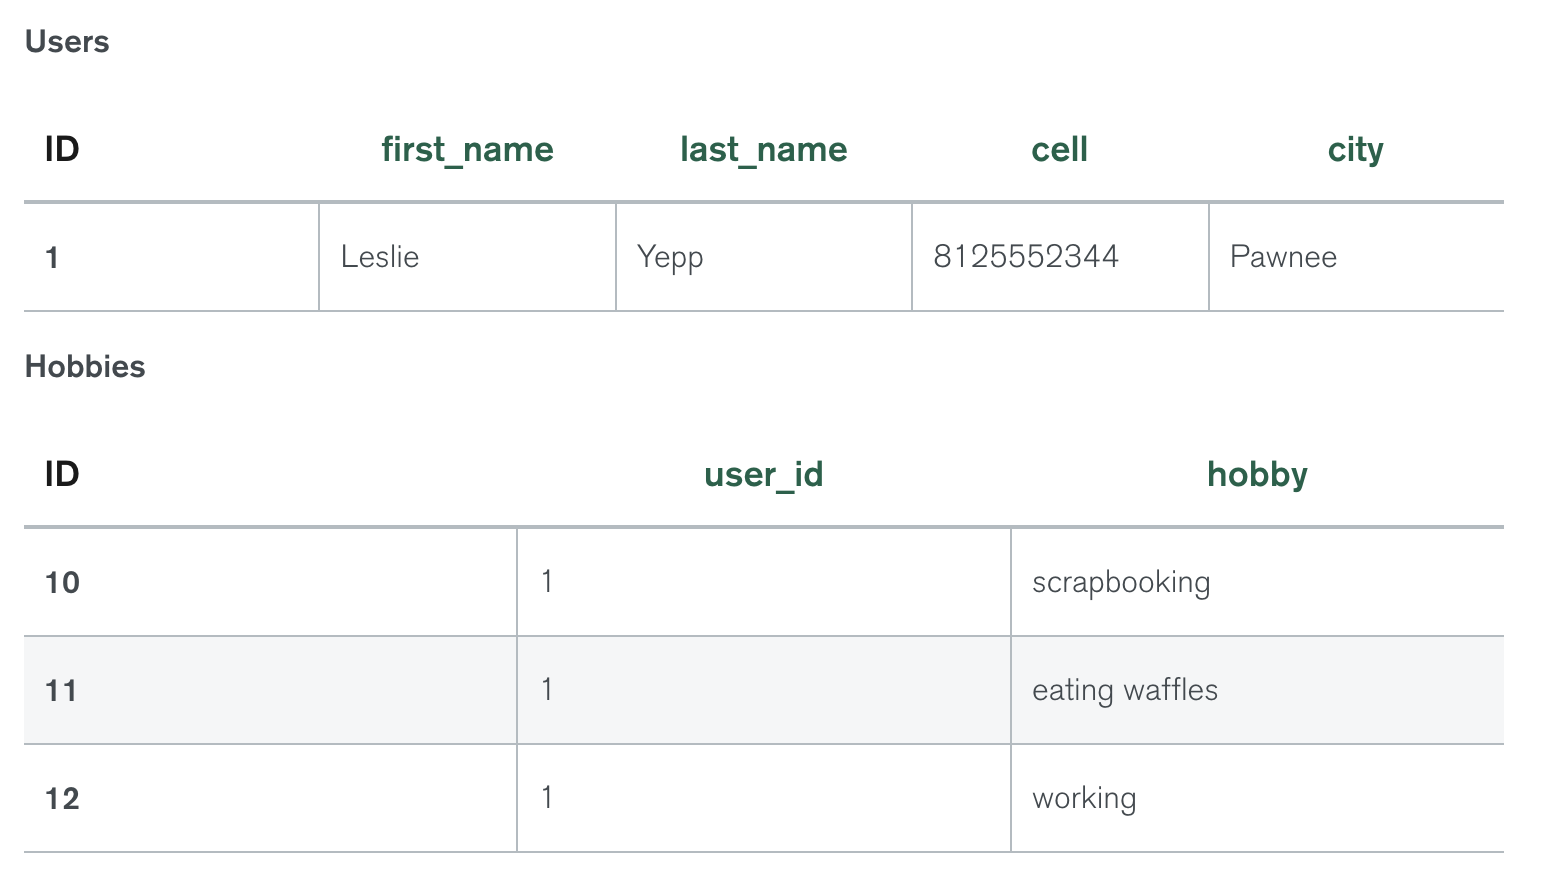
\includegraphics[width=1\textwidth]{gambar/pemodelan_rdbms.png}
	\captionsource{Pemodelan RDBMS}{\href{https://www.mongodb.com/nosql-explained}{\textit{https://www.mongodb.com/nosql-explained}}}
	\label{fig:pemodelan_rdbms}
\end{figure}
\begin{figure}[H]
	\centering
	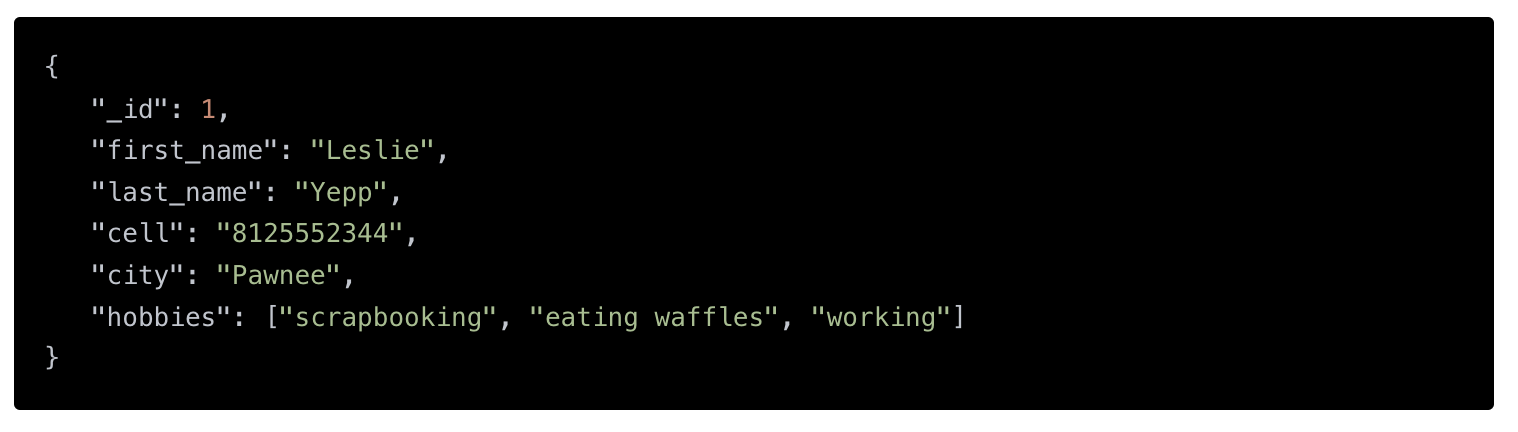
\includegraphics[width=1\textwidth]{gambar/pemodelan_nosql.png}
	\captionsource{Pemodelan NoSQL}{\href{https://www.mongodb.com/nosql-explained}{\textit{https://www.mongodb.com/nosql-explained}}}
	\label{fig:pemodelan_nosql}
\end{figure}
	
	Menurut Gambar \ref{fig:pemodelan_rdbms}, untuk menyimpan data \textit{user} dan data \textit{hobby}, diperlukan dua tabel terpisah, sedangkan dalam pemodelan NoSQL Gambar \ref{fig:pemodelan_nosql}, data \textit{user} dan \textit{hobby} dalam satu dokumen yang sama. Dengan NoSQL, ketika ingin mengambil dua bagian data secara bersamaan, hanya memerlukan satu dokumen tanpa gabungan, yang menghasilkan kueri lebih cepat daripada RDBMS.
	
	Meskipun NoSQL, desain database masih harus dilakukan. Desain basis data memungkinkan untuk mengonfirmasi dan mendokumentasikan pemahaman tentang basis data dan memastikan bahwa orang-orang melihat lanskap informasi dengan cara yang sama. Dengan kata lain, desain database adalah alat komunikasi. Berikut merupakan komparasi dari RDBMS dan NoSQL \textbf{Table \ref{table:komparasi_database}} \citep{Kunda2017ACS}.
	
	
\begin{table}[H]
	\centering
	\caption{\textit{Komparasi Database RDBMS dan NoSQL}}
	\label{table:komparasi_database}
	\begin{tabular}{@{} |p{0.5cm}|p{2cm}|p{5cm}|p{5cm}| @{}}
		\hline
		\textbf{No} & \textbf{Kriteria} & \textbf{RDBMS} & \textbf{NoSQL} \\
		\hline
		1 & Variety &  Terdapat dalam jenis open source dan close platform & Kebanyakan dalam bentuk open source\\
		\hline
		2 & Scalability &  Meningkatkan performa dengan meningkatkan hardware dalam server & Meningkatkan dengan cara horizontal atau menambah server\\
		\hline
		3 & Cost &  Lebih mahal mengingat harusnya penambahan hardware & Lebih murah mengingat murahnya upgrade secara horizontal \\
		\hline
		4 & Volume of Data &  Menangani data yang terbatas & Menangani data yang lebih besar\\
		\hline
		5 & Performance &  Lebih lambat karena perlunya memproses informasi  & Memiliki query performance lebih baik\\
		\hline
		6 & Complexity &  Lebih kompleks karena memerlukan normalisasi hubungan antara tabel & lebih flexible dapat menyimpan struktur yang berbeda dalam satu collections\\
		\hline
		7 & Consistency &  Dengan skema yang kompleks menjadikannya lebih konsisten & Kurang konsisten dikarenakan skema yang bermacam-macam\\
		\hline
		8 & Security &  Memiliki mekanisme keamanan yang baik untuk melindungi data & Keamanan ditangani oleh middleware dan bukan bagian dari database\\
		\hline
	\end{tabular}
\end{table}

\section{Flask Framework}

Framework adalah kerangka kerja untuk mengembangkan aplikasi berbasis web dan desktop. Kerangka kerja di sini sangat membantu pengembang untuk menulis hal-hal yang lebih terstruktur dan rapi.

Framework ini dibuat untuk menyederhanakan kinerja bagi pemrogram. Jadi programmer tidak perlu menulis kode berulang-ulang. Karena hanya perlu mengkompilasi komponen pemrograman itu sendiri \citep{robithadani2020framework}.

Flask Framework merupakan kerangka kerja yang berbasis web. Flask dibangun diatas bahasa pemrograman python dengan menggunakan dependensi Werkzeug dan Jinja2. Kerangka kerja Flask bersifat mikro karena tidak membutuhkan alat-alat tertentu atau pustaka. Flask mendukung ekstensi yang dapat menambahkan fitur aplikasi seolah-olah mereka diimplementasikan dalam Flask itu sendiri.
	
	
	\subsection {Flask routing}
	
	Routing adalah modul dalam aplikasi yang mengatur pengoperasian aplikasi berbasis web. Route dapat menangani semua perintah yang telah  dideklarasikan. Routing bisa dianalogikan sebagai route diagram penjelas tentang cara menavigasi aplikasi yang sedang dibangun.
	
	App Routing berarti memetakan URL ke fungsi tertentu yang akan menangani logika untuk URL tersebut. Berikut adalah contoh routing di framework flask:

\begin{lstlisting}
from flask import Flask
  
app = Flask(__name__)
  
# Pass the required route to the decorator.
@app.route("/hello")
def hello():
   	return "Hello, Welcome to GeeksForGeeks"
    
@app.route("/")
def index():
    	return "Homepage of GeeksForGeeks"
  
if __name__ == "__main__":
	app.run(debug=True)
\end{lstlisting}

Seperti potongan code di atas pemetaan URL ke fungsi menggunakan decorator sebelum fungsi ditulis. Dan contoh diatas merupakan contoh yang sederhana pada routing. Berikut adalah beberapa hal yang bisa dilakukan flask routing:

\begin{enumerate}[a.]
	\item Route Methods
		
		Pada dasarnya saat melakukan routing, secara default metode yang dipakai adalah GET. Untuk membuat agar URL dapat menggunakan metode lain seperti POST diharuskan mendefinisikan metodenya pada argumen route.
\begin{lstlisting}
@app.route('/home', methods=['POST', 'GET']) 
def home(): 
    return '<h1>Anda berada di halaman beranda!</h1>'
\end{lstlisting}
	\item Route Variables
		
		Meneruskan variables merupakan sebuah fitur dasar yang memungkinkan pengguna mengirimkan informasi melalui URL. Untuk mengimplementasikan fitur ini route harus mendefinisikan variabel tersebut dalam URL dan menjadikannya argumen pada fungsinya \citep{meissamrasouli2020flaskroute}.
\begin{lstlisting}
@app.route('/home/<firstname>', methods=['POST', 'GET']) 
def home(firstname): 
    return '<h1>Halo {}, Anda berada di halaman beranda!</ h1>'.format(nama depan)
\end{lstlisting}
\end{enumerate}
		
	\subsection {Dependencies}
	
		Dependencies merupakan ketergantungan suatu sistem kepada sistem lainnya. Dalam halnya framework, ketergantungannya adalah terhadap sebuah package atau extension. Package atau extension berisi sebuah resource suatu logic yang bisa diimplementasikan dengan mudah dengan hanya memanggil package tersebut yang biasanya berbentuk object class.
		
	\begin{enumerate}[a.]
		\item{Flask-REStful}
		
		Flask-REStful merupakan extension untuk framework Flask untuk membantu membangun REST API dengan cepat. Flask-REStful mengedepankan peraktek terbaik dengan pengaturan yang diminimalkan \citep{kevinburke2020flaskrestful}.
		
		Pengimplementasian Flask-REStful dimulai dengan penginstalan dengan cara
\begin{lstlisting}
pip install flask-restful
\end{lstlisting}
		dilanjutkan dengan menggunakan import Resource dan Api dari Flask-REStful, buat variabel yang akan menyimpan sebuah class Api dengan argumen Flask, kemudian buat class child dari sebuah class Resource, pada setiap class sudah dapat menerapkan fungsi dari parent Resource seperti get, post, put, dll, kemudian adalah tambahkan mapping class tersebut kepada string endpoint URL.
\begin{lstlisting}[language=Python, caption=Python example]
from flask import Flask
from flask_restful import Resource, Api

app = Flask(__name__)
api = Api(app)

class HelloWorld(Resource):
    def get(self):
        return {'hello': 'world'}

api.add_resource(HelloWorld, '/')

if __name__ == '__main__':
    app.run(debug=True)
\end{lstlisting}

		
		\item{Flask-Mongoengine}
		
		Flask-Mongoengine merupakan extension Flask yang menyediakan integrasi Flask ke MongoEngine. MongoEngine sendiri merupakan library python yang berperan sebagai Object Document Mapper dengan MongoDB \citep{streetlife2020flaskmongoenginedocumentation}.
		
		Pengimplementasian Flask-Mongoengine dimulai dengan penginstalan dengan cara 
\begin{lstlisting}
pip install flask-mongoengine
\end{lstlisting}
		dilanjutkan dengan import Mongoengine dari Flask-Mongoengine, lakukan inisiasi untuk app Flask, gunakan fungsi ".config" untuk melakukan konfigurasi database yang akan di pakai, lalu inisiasi MongoEngine dan gunakan fungsi "init\_app" dengan memasukkan parameter app Flask.
\begin{lstlisting}
import flask
from flask_mongoengine import MongoEngine
		

db = MongoEngine()
app = flask.Flask("example_app")
app.config["MONGODB_SETTINGS"] = [
    {
        "db": "project1",
        "host": "localhost",
        "port": 27017,
        "alias": "default",
    }
]
db.init_app(app)
\end{lstlisting}

		Penggunaan MongoEngine diawali dengan mendefinisikan dokumen yang akan di simpan dalam bentuk class yang memiliki parent Document. Mendefinisikan dokumen juga mengharuskan kita mendefinisikan field yang ada didalamnya dengan menetapkannya sebagai property class dan menetapkan jenis dari setiap property class tersebut \citep{rosslawley2020mongoeingedocumentation}.
\begin{lstlisting}
from mongoengine import *
import datetime

class Page(Document):
    title = StringField(max_length=200, required=True)
    date_modified = DateTimeField(default=datetime.datetime.utcnow)
\end{lstlisting}

		Setelah Pendefinisian dokumen, memanipulasi data dapat dilakukan dengan memanggil fungsi pada class tersebut. Berikut merupakan contoh dari manipulasi data pada Mongoengine.
		
\begin{lstlisting}
from mongoengine import *

#Saving Documents
page = Page(title="Test Page")
page.save()
id = page.id

#Update Documents with id
page2 = Page.objects.get(id=id)
page2.update({title: "Test 123"})

#Delete Documents with id
page3 = Page.objects.get(id=id)
page3.delete()

\end{lstlisting}
		
	\end{enumerate}
	
		

\section{Apache}
	
	Apache adalah perangkat lunak server yang dapat digunakan untuk membuat koneksi antara browser web dan server menggunakan protokol HyperText Transfer, atau HTTP. Apache memiliki fitur yang cukup untuk melakukan konfigurasi dasar seperti pesan kesalahan dan otentikasi berbasis database. Saat digunakan, itu akan membuat kumpulan proses, atau daemon, untuk menangani permintaan. Arsitektur Apache didasarkan pada model client-server berbasis thread yang menggunakan modul; modul ini termasuk keamanan, penulisan ulang URL dan otentikasi kata sandi antara lain \citep{apachehttpserver2022}.

	\subsection{Konfigurasi httpd.conf}
	
		Konfigurasi Apache pada server adalah dengan mendaftarkan Aplikasi pada file httpd.conf. Berikut merupakan contoh pendaftaran pada httpd.conf

\begin{lstlisting}
WSGIDaemonProcess /fishapi python-path=/opt/rh/rh-python38/root/lib/pyt$
WSGIProcessGroup /fishapi
WSGIApplicationGroup %{GLOBAL}
WSGIScriptAlias /fishapi /var/www/html/fishapi/index.wsgi
WSGIScriptReloading on
<Directory "/var/www/html/fishapi/fishapi">
	AllowOverride All
	Options +ExecCGI
	AddHandler cgi-script .cgi .pl .py
	Order allow,deny
	allow from all
</Directory>

Alias /fishapi/static /var/www/html/fishapi/fishapi/static
<Directory /var/www/html/fishapi/fishapi/static>
	AllowOverride All
	Order allow,deny
	allow from all
</Directory>
\end{lstlisting}
		
\section{Unit Testing}
Unit testing merupakan salah satu tipe pengujian perangkat lunak dimana setiap fungsi atau komponen dari perangkat lunak diuji. Tujuan dari unit testing adalah untuk memastikan fungsi pada perangkat lunak sudah berjalan sesuai dengan ekspetasi \citep{hamilton2022unittesting}. Menurut \citep{rosa2016rekayasa},“Unit testing berfokus pada pengujian unit terkecil (komponen perangkat lunak atau modul) dari desain perangkat lunak. Semua fungsi pada perangkat lunak diuji untuk memastikan bahwa input dan output unit sesuai dengan yang diinginkan”.

Teknik yang dilakukan pada unit testing adalah “berfokus pada setiap unit perangkat lunak (misalnya komponen, kelas, atau objek konten dari aplikasi atau web) seperti yang diterapkan dalam kode program” \citep{pressman2012}. Kode program dikaji apakah terdapat kesalahan. Kesalahan pada kode program dapat diidentifikasi dengan menggunakan White-Box Testing. Sedangkan menurut \citep{rosa2016rekayasa}, “White-Box Testing (pengujian kotak putih) merupakan pengujian perangkat lunak atau aplikasi dari segi desain dan kode program untuk mengetahui apakah perangkat lunak mampu menghasilkan fungsi- fungsi, masukan, dan keluaran yang sesuai dengan spesifikasi kebutuhan”.

Proses unit testing memastikan fungsi-fungsi pada aplikasi yang telah dikembangkan peneliti memenuhi persyaratan, dapat berjalan dengan baik, dan memiliki input serta output sesuai yang diinginkan. Berdasarkan definisi di atas dapat disimpulkan bahwa unit testing merupakan salah satu tipe pengujian fungsi atau unit pada perangkat lunak untuk memastikan apakah perangkat lunak mampu untuk menghasilkan input dan output sesuai dengan spesifikasi yang telah ditentukan.


\section{User Acceptance Test (UAT)}
Menurut \citep{perry2006effectivemethods} User Acceptance Test (UAT) yaitu pengujian untuk verifikasi apakah fungsi pada sistem telah berjalan dengan kebutuhan, pengujian dilakukan oleh user dimana user tersebut adalah staff/karyawan perusahaan yang langsung berinteraksi dengan sistem. Menurut Black, acceptance testing pada umumnya menunjukkan bahwa sistem telah memenuhi persyaratan-persyaratan tertentu. Pada pengembangan software dan hardware komersial, acceptance test biasanya disebut juga "alpha tests" (yang dilakukan oleh pengguna in-house) dan "beta tests" (yang dilakukan oleh pengguna yang sedang menggunakan atau akan menggunakan sistem tersebut). 

Menurut \citep{hady2020user} menyebutkan bahwa pelaksanaan UAT terdapat pada akhir proses pengujian saat sistem siap digunakan. Tujuan utama UAT adalah untuk memvalidasi apakah sistem diterima atau ditolak, memenuhi spesifikasi sistem, dan mengembangkan perangkat lunak yang mampu memenuhi kebutuhan user. 

Proses UAT memastikan bahwa web service berjalan dapat berjalan dengan baik, mengembalikan respon sesuai kebutuhan bagi kepentingan pengembangan frontend. Dari definisi yang telah dipaparkan dapat disimpulkan bahwa UAT adalah pengujian pada akhir proses yang dilakukan oleh pengguna pada sebuah sistem untuk memastikan fungsi-fungsi yang terdapat pada sistem tersebut telah berjalan dengan baik dan sesuai dengan kebutuhan pengguna.

\section{Black box testing}
Black Box Testing adalah salah satu metode pengujian perangkat lunak yang berfokus pada menguji fungsionalitas dari suatu aplikasi atau sistem tanpa memperhatikan bagaimana implementasi internal dari kode tersebut. Dalam black box testing, pengujian dilakukan berdasarkan input yang diberikan kepada sistem dan keluaran atau respons yang dihasilkan oleh sistem, tanpa memperhatikan detail bagaimana sistem melakukan prosesnya.

Dalam black box testing, seorang tester menganggap sistem sebagai "kotak hitam" di mana mereka hanya memiliki informasi mengenai input yang harus diberikan dan keluaran yang seharusnya dihasilkan. Tujuannya adalah untuk memastikan bahwa sistem memberikan hasil yang sesuai dengan harapan pengguna, sesuai dengan persyaratan yang telah ditetapkan, tanpa harus mengetahui bagaimana sistem mencapai hasil tersebut.
		

% Baris ini digunakan untuk membantu dalam melakukan sitasi
% Karena diapit dengan comment, maka baris ini akan diabaikan
% oleh compiler LaTeX.
\begin{comment}
\bibliography{daftar-pustaka}
\end{comment}